
% This LaTeX was auto-generated from MATLAB code.
% To make changes, update the MATLAB code and republish this document.

\documentclass{article}
\usepackage{graphicx}
\usepackage{color}

\sloppy
\definecolor{lightgray}{gray}{0.5}
\setlength{\parindent}{0pt}

\begin{document}

    
    
\section*{Accelerated Gradient Descent}


\subsection*{Contents}

\begin{itemize}
\setlength{\itemsep}{-1ex}
   \item Gradient
   \item Gradient Descent
   \item Accelerated Gradient Descent
   \item Plot contour
   \item Reference
\end{itemize}


\subsection*{Gradient}

\begin{par}
Gradient descent method is based on gradient
\end{par} \vspace{1em}
\begin{par}
$$ \nabla f  = \frac{\partial f}{\partial x_1 }\mathbf{e}_1 + \cdots +
\frac{\partial f}{\partial x_n }\mathbf{e}_n $$
\end{par} \vspace{1em}
\begin{par}
gradient always point to the asent direction
\end{par} \vspace{1em}


\subsection*{Gradient Descent}

\begin{par}
f is object function, and this is unconstrained
\end{par} \vspace{1em}
\begin{par}
$$\min_{x} f $$
\end{par} \vspace{1em}


\subsection*{Accelerated Gradient Descent}

\begin{par}
for t = 1,2,...
\end{par} \vspace{1em}
\begin{par}
$$x^{(t)} = y^{(t-1)} - alpha \nabla f(y^{t-1})$$
\end{par} \vspace{1em}
\begin{par}
$$y^{(t)} = x^{(t)} + (t-1) / (t+2) * (x^{(t)} - x^{(t-1)})$$
\end{par} \vspace{1em}
\begin{verbatim}
f = (@(X) (exp(X(1,:)-1) + exp(1-X(2,:)) + (X(1,:) - X(2,:)).^2));
%f = (@(X) (sin(0.5*X(1,:).^2 - 0.25 * X(2,:).^2 + 3) .* cos(2*X(1,:) + 1 - exp(X(2,:))) ))
\end{verbatim}


\subsection*{Plot contour}

\begin{verbatim}
[X, Y] = meshgrid(-2:0.1:2);
XX = [reshape(X, 1, numel(X)); reshape(Y, 1, numel(Y))];
%surf(X, Y, reshape(f(XX), length(X), length(X)))
contour(X, Y, reshape(f(XX), length(X), length(X)), 50);

hold on;
\end{verbatim}

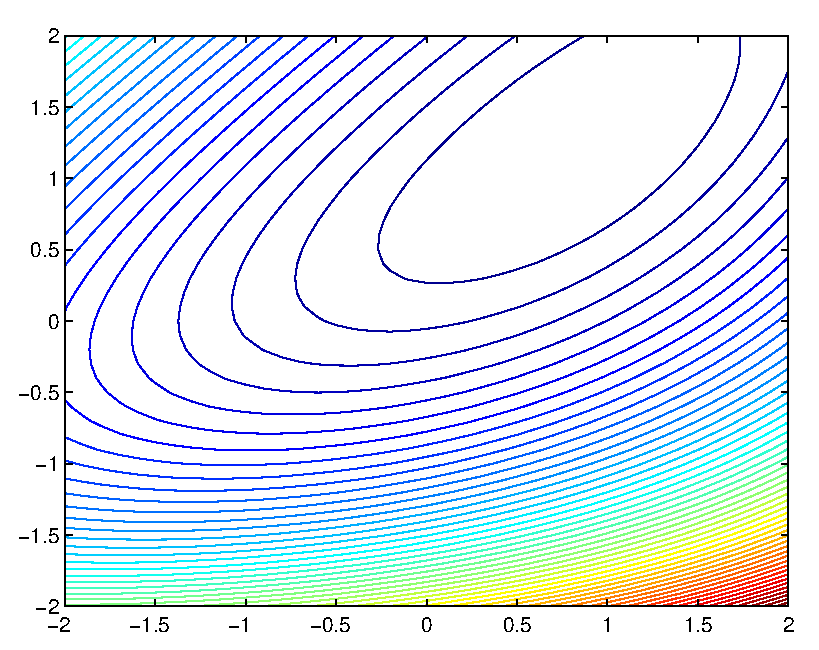
\includegraphics [width=4in]{test_01.eps}
\begin{par}
plot gradient of function
\end{par} \vspace{1em}
\begin{verbatim}
for i=1:5:length(XX)
    tmp = XX(:,i);
    g = gradient_of_function(f, tmp);
    %plot([tmp(1),tmp(1)+g(1)*0.02],[tmp(1),tmp(2)+g(1)*0.02]);
    quiver(tmp(1),tmp(2),g(1)*0.02,g(2)*0.02);
end
\end{verbatim}

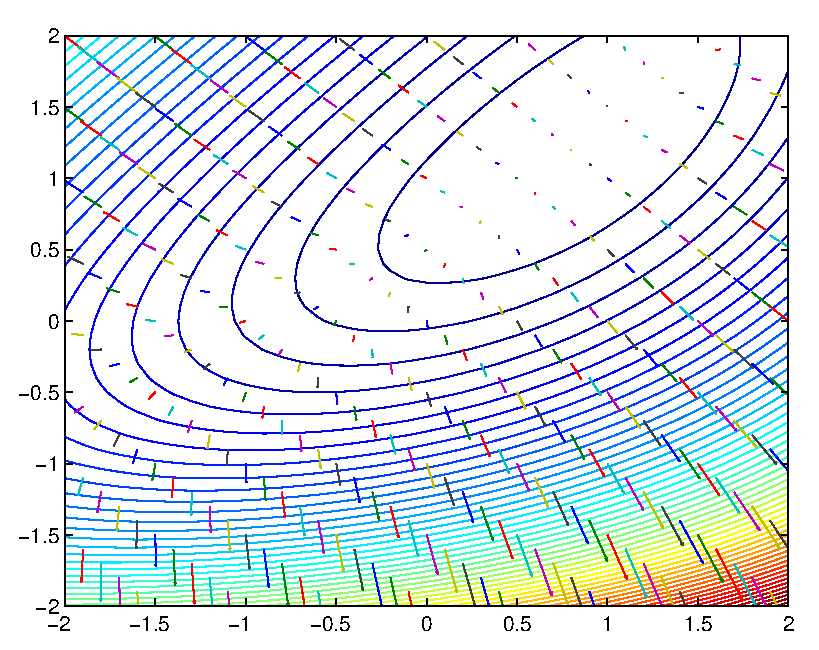
\includegraphics [width=4in]{test_02.eps}
\begin{par}
calculation
\end{par} \vspace{1em}
\begin{verbatim}
x0 = [-1; -1];
\end{verbatim}
\begin{par}
without wolfe step, fix step as alpha = 0.01, $x_k = x_{k-1} + alpha * (-\nabla f)$
\end{par} \vspace{1em}
\begin{verbatim}
[x_gf, v_gf, h_gf] = gradient_fix_step(f, x0)
[x_af, v_af, h_af] = accelerated_gradient_fix_step(f, x0)
\end{verbatim}

        \color{lightgray} \begin{verbatim}
x_gf =

   -0.0287
    0.5194


v_gf =

    2.2750


h_gf =

  Columns 1 through 7

   -1.0000   -1.0014   -1.0012   -0.9997   -0.9970   -0.9933   -0.9886
   -1.0000   -0.9261   -0.8590   -0.7977   -0.7413   -0.6894   -0.6413

  Columns 8 through 14

   -0.9830   -0.9766   -0.9696   -0.9619   -0.9537   -0.9449   -0.9357
   -0.5966   -0.5550   -0.5161   -0.4796   -0.4454   -0.4131   -0.3826

  Columns 15 through 21

   -0.9261   -0.9161   -0.9058   -0.8952   -0.8843   -0.8732   -0.8619
   -0.3538   -0.3266   -0.3007   -0.2761   -0.2526   -0.2303   -0.2089

  Columns 22 through 28

   -0.8503   -0.8387   -0.8269   -0.8150   -0.8029   -0.7908   -0.7786
   -0.1885   -0.1689   -0.1501   -0.1320   -0.1147   -0.0980   -0.0818

  Columns 29 through 35

   -0.7664   -0.7541   -0.7418   -0.7294   -0.7170   -0.7047   -0.6923
   -0.0663   -0.0512   -0.0367   -0.0226   -0.0089    0.0044    0.0172

  Columns 36 through 42

   -0.6800   -0.6676   -0.6553   -0.6431   -0.6308   -0.6186   -0.6065
    0.0298    0.0420    0.0538    0.0654    0.0767    0.0877    0.0985

  Columns 43 through 49

   -0.5944   -0.5823   -0.5704   -0.5585   -0.5466   -0.5348   -0.5231
    0.1090    0.1193    0.1294    0.1393    0.1490    0.1585    0.1678

  Columns 50 through 56

   -0.5115   -0.4999   -0.4884   -0.4770   -0.4657   -0.4544   -0.4433
    0.1770    0.1860    0.1949    0.2036    0.2121    0.2206    0.2289

  Columns 57 through 63

   -0.4322   -0.4212   -0.4103   -0.3995   -0.3887   -0.3781   -0.3675
    0.2370    0.2451    0.2531    0.2609    0.2686    0.2763    0.2838

  Columns 64 through 70

   -0.3570   -0.3466   -0.3363   -0.3261   -0.3160   -0.3059   -0.2960
    0.2912    0.2986    0.3058    0.3130    0.3201    0.3271    0.3341

  Columns 71 through 77

   -0.2861   -0.2764   -0.2667   -0.2571   -0.2475   -0.2381   -0.2288
    0.3409    0.3477    0.3544    0.3611    0.3677    0.3742    0.3806

  Columns 78 through 84

   -0.2195   -0.2103   -0.2012   -0.1922   -0.1833   -0.1745   -0.1657
    0.3870    0.3933    0.3996    0.4058    0.4120    0.4181    0.4241

  Columns 85 through 91

   -0.1570   -0.1484   -0.1399   -0.1315   -0.1231   -0.1148   -0.1066
    0.4301    0.4361    0.4419    0.4478    0.4536    0.4593    0.4650

  Columns 92 through 98

   -0.0985   -0.0904   -0.0825   -0.0746   -0.0668   -0.0590   -0.0513
    0.4706    0.4762    0.4818    0.4873    0.4927    0.4982    0.5035

  Columns 99 through 101

   -0.0437   -0.0362   -0.0287
    0.5089    0.5142    0.5194


x_af =

    0.7415
    1.1499


v_af =

    1.7998


h_af =

  Columns 1 through 7

   -1.0000   -1.0014   -1.0012   -0.9993   -0.9950   -0.9875   -0.9761
   -1.0000   -0.9261   -0.8590   -0.7823   -0.6989   -0.6115   -0.5223

  Columns 8 through 14

   -0.9604   -0.9398   -0.9140   -0.8829   -0.8463   -0.8043   -0.7571
   -0.4333   -0.3459   -0.2615   -0.1807   -0.1043   -0.0325    0.0345

  Columns 15 through 21

   -0.7050   -0.6484   -0.5877   -0.5234   -0.4562   -0.3866   -0.3154
    0.0969    0.1548    0.2086    0.2587    0.3057    0.3499    0.3920

  Columns 22 through 28

   -0.2430   -0.1703   -0.0976   -0.0257    0.0449    0.1139    0.1807
    0.4324    0.4716    0.5100    0.5481    0.5861    0.6242    0.6627

  Columns 29 through 35

    0.2451    0.3067    0.3654    0.4209    0.4732    0.5223    0.5680
    0.7016    0.7410    0.7807    0.8208    0.8611    0.9013    0.9413

  Columns 36 through 42

    0.6106    0.6500    0.6864    0.7198    0.7505    0.7786    0.8042
    0.9809    1.0197    1.0575    1.0941    1.1292    1.1626    1.1940

  Columns 43 through 49

    0.8276    0.8487    0.8679    0.8851    0.9005    0.9142    0.9262
    1.2234    1.2505    1.2752    1.2975    1.3174    1.3346    1.3494

  Columns 50 through 56

    0.9366    0.9455    0.9528    0.9587    0.9631    0.9661    0.9677
    1.3618    1.3718    1.3794    1.3849    1.3884    1.3899    1.3897

  Columns 57 through 63

    0.9679    0.9667    0.9643    0.9606    0.9558    0.9499    0.9429
    1.3878    1.3845    1.3798    1.3740    1.3672    1.3595    1.3510

  Columns 64 through 70

    0.9350    0.9263    0.9169    0.9069    0.8964    0.8855    0.8743
    1.3419    1.3322    1.3222    1.3118    1.3012    1.2904    1.2795

  Columns 71 through 77

    0.8630    0.8517    0.8404    0.8293    0.8185    0.8080    0.7979
    1.2686    1.2578    1.2471    1.2366    1.2263    1.2163    1.2067

  Columns 78 through 84

    0.7883    0.7793    0.7708    0.7629    0.7557    0.7492    0.7433
    1.1974    1.1886    1.1803    1.1725    1.1653    1.1587    1.1527

  Columns 85 through 91

    0.7382    0.7337    0.7300    0.7269    0.7246    0.7229    0.7218
    1.1474    1.1428    1.1388    1.1356    1.1330    1.1312    1.1300

  Columns 92 through 98

    0.7214    0.7216    0.7224    0.7237    0.7256    0.7279    0.7307
    1.1295    1.1296    1.1304    1.1317    1.1336    1.1361    1.1389

  Columns 99 through 101

    0.7339    0.7375    0.7415
    1.1422    1.1459    1.1499

\end{verbatim} \color{black}
    \begin{par}
find suitable step size
\end{par} \vspace{1em}
\begin{verbatim}
[x_g, v_g, h_g] = gradient(f, x0)
[x_a, v_a, h_ax, h_ay] = accelerated_gradient(f, x0)


% built-in method
[x_in, v_in] = fminunc(f, x0)
\end{verbatim}

        \color{lightgray} \begin{verbatim}
x_g =

    0.7960
    1.2038


v_g =

    1.7974


h_g =

  Columns 1 through 7

   -1.0000   -1.0271   -0.4515    0.6432    0.8185    0.7755    0.7859
   -1.0000    0.4778    0.2130    1.0809    1.1279    1.1801    1.2059

  Columns 8 through 12

    0.7925    0.7963    0.7956    0.7959    0.7960
    1.2007    1.2024    1.2033    1.2039    1.2038


x_a =

    0.7960
    1.2038


v_a =

    1.7974


h_ax =

  Columns 1 through 7

   -1.0000   -1.0169    0.7311    1.0381    1.0156    1.0217    0.9513
   -1.0000   -0.0764    0.9765    1.3202    1.4675    1.4183    1.3769

  Columns 8 through 14

    0.9013    0.8435    0.8050    0.7829    0.7738    0.7789    0.7808
    1.3051    1.2559    1.2170    1.1899    1.1882    1.1842    1.1906

  Columns 15 through 21

    0.7879    0.7930    0.7966    0.7966    0.7968    0.7971    0.7968
    1.1945    1.1993    1.2037    1.2046    1.2050    1.2048    1.2047

  Columns 22 through 25

    0.7966    0.7963    0.7961    0.7960
    1.2043    1.2040    1.2038    1.2038


h_ay =

  Columns 1 through 7

   -1.0000   -1.0169    1.1681    1.1609    1.0044    1.0251    0.9073
   -1.0000   -0.0764    1.2398    1.4577    1.5411    1.3902    1.3510

  Columns 8 through 14

    0.8679    0.8031    0.7770    0.7662    0.7668    0.7829    0.7823
    1.2573    1.2214    1.1888    1.1695    1.1870    1.1811    1.1956

  Columns 15 through 21

    0.7936    0.7972    0.7997    0.7966    0.7970    0.7973    0.7965
    1.1978    1.2032    1.2074    1.2054    1.2053    1.2045    1.2046

  Columns 22 through 25

    0.7964    0.7961    0.7959    0.7960
    1.2040    1.2038    1.2036    1.2039

Warning: Gradient must be provided for trust-region algorithm;
  using line-search algorithm instead. 

Local minimum found.

Optimization completed because the size of the gradient is less than
the default value of the function tolerance.




x_in =

    0.7961
    1.2039


v_in =

    1.7974

\end{verbatim} \color{black}
    \begin{par}
plot descent steps
\end{par} \vspace{1em}
\begin{verbatim}
for i=2:length(h_gf)
    tmp1 = h_gf(:,i-1);
    tmp2 = h_gf(:,i);
    quiver(tmp1(1),tmp1(2),tmp2(1)-tmp1(1),tmp2(2)-tmp1(2), 0, 'g','LineWidth',3)
end


for i=2:length(h_af)
    tmp1 = h_af(:,i-1);
    tmp2 = h_af(:,i);
    quiver(tmp1(1),tmp1(2),tmp2(1)-tmp1(1),tmp2(2)-tmp1(2), 0, 'b','LineWidth',3)
end


for i=2:length(h_g)
    tmp1 = h_g(:,i-1);
    tmp2 = h_g(:,i);
    quiver(tmp1(1),tmp1(2),tmp2(1)-tmp1(1),tmp2(2)-tmp1(2), 0, 'r','LineWidth',2)
end

for i=2:length(h_ax)
    tmp1 = h_ax(:,i-1);
    tmp2 = h_ax(:,i);
    quiver(tmp1(1),tmp1(2),tmp2(1)-tmp1(1),tmp2(2)-tmp1(2), 0, 'c','LineWidth',2)
end

for i=2:length(h_ay)
    tmp1 = h_ay(:,i-1);
    tmp2 = h_ay(:,i);
    quiver(tmp1(1),tmp1(2),tmp2(1)-tmp1(1),tmp2(2)-tmp1(2), 0, 'm','LineWidth',2)
end
\end{verbatim}

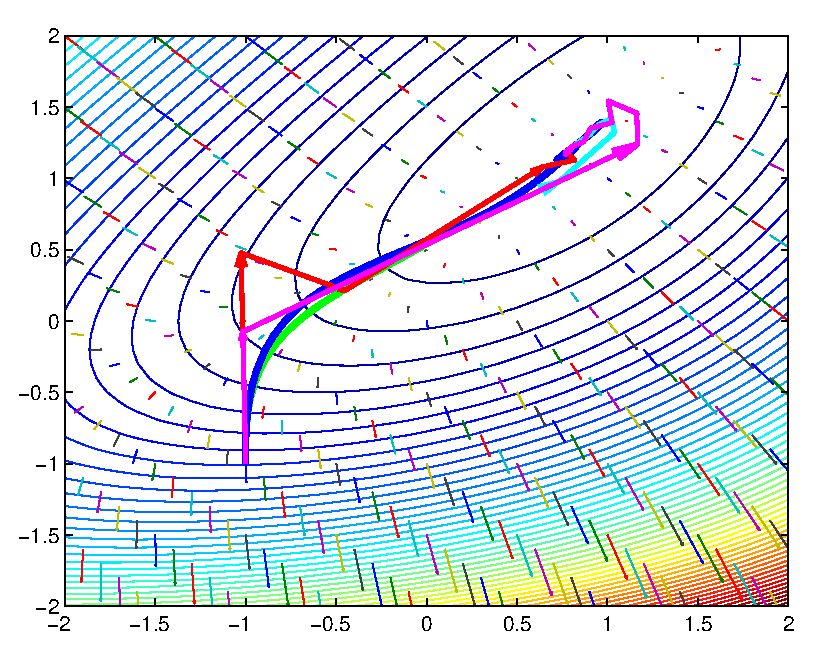
\includegraphics [width=4in]{test_03.eps}


\subsection*{Reference}

\begin{enumerate}
\setlength{\itemsep}{-1ex}
   \item \begin{verbatim}http://stronglyconvex.com/blog/accelerated-gradient-descent.html\end{verbatim}
\end{enumerate}



\end{document}
    
